% Chapter Template

\chapter{Results} % Main chapter title

\label{Chapter4} % Change X to a consecutive number; for referencing this chapter elsewhere, use \ref{ChapterX}

%----------------------------------------------------------------------------------------
%	SECTION 1
%----------------------------------------------------------------------------------------
\begin{figure}[!htb]
\centering
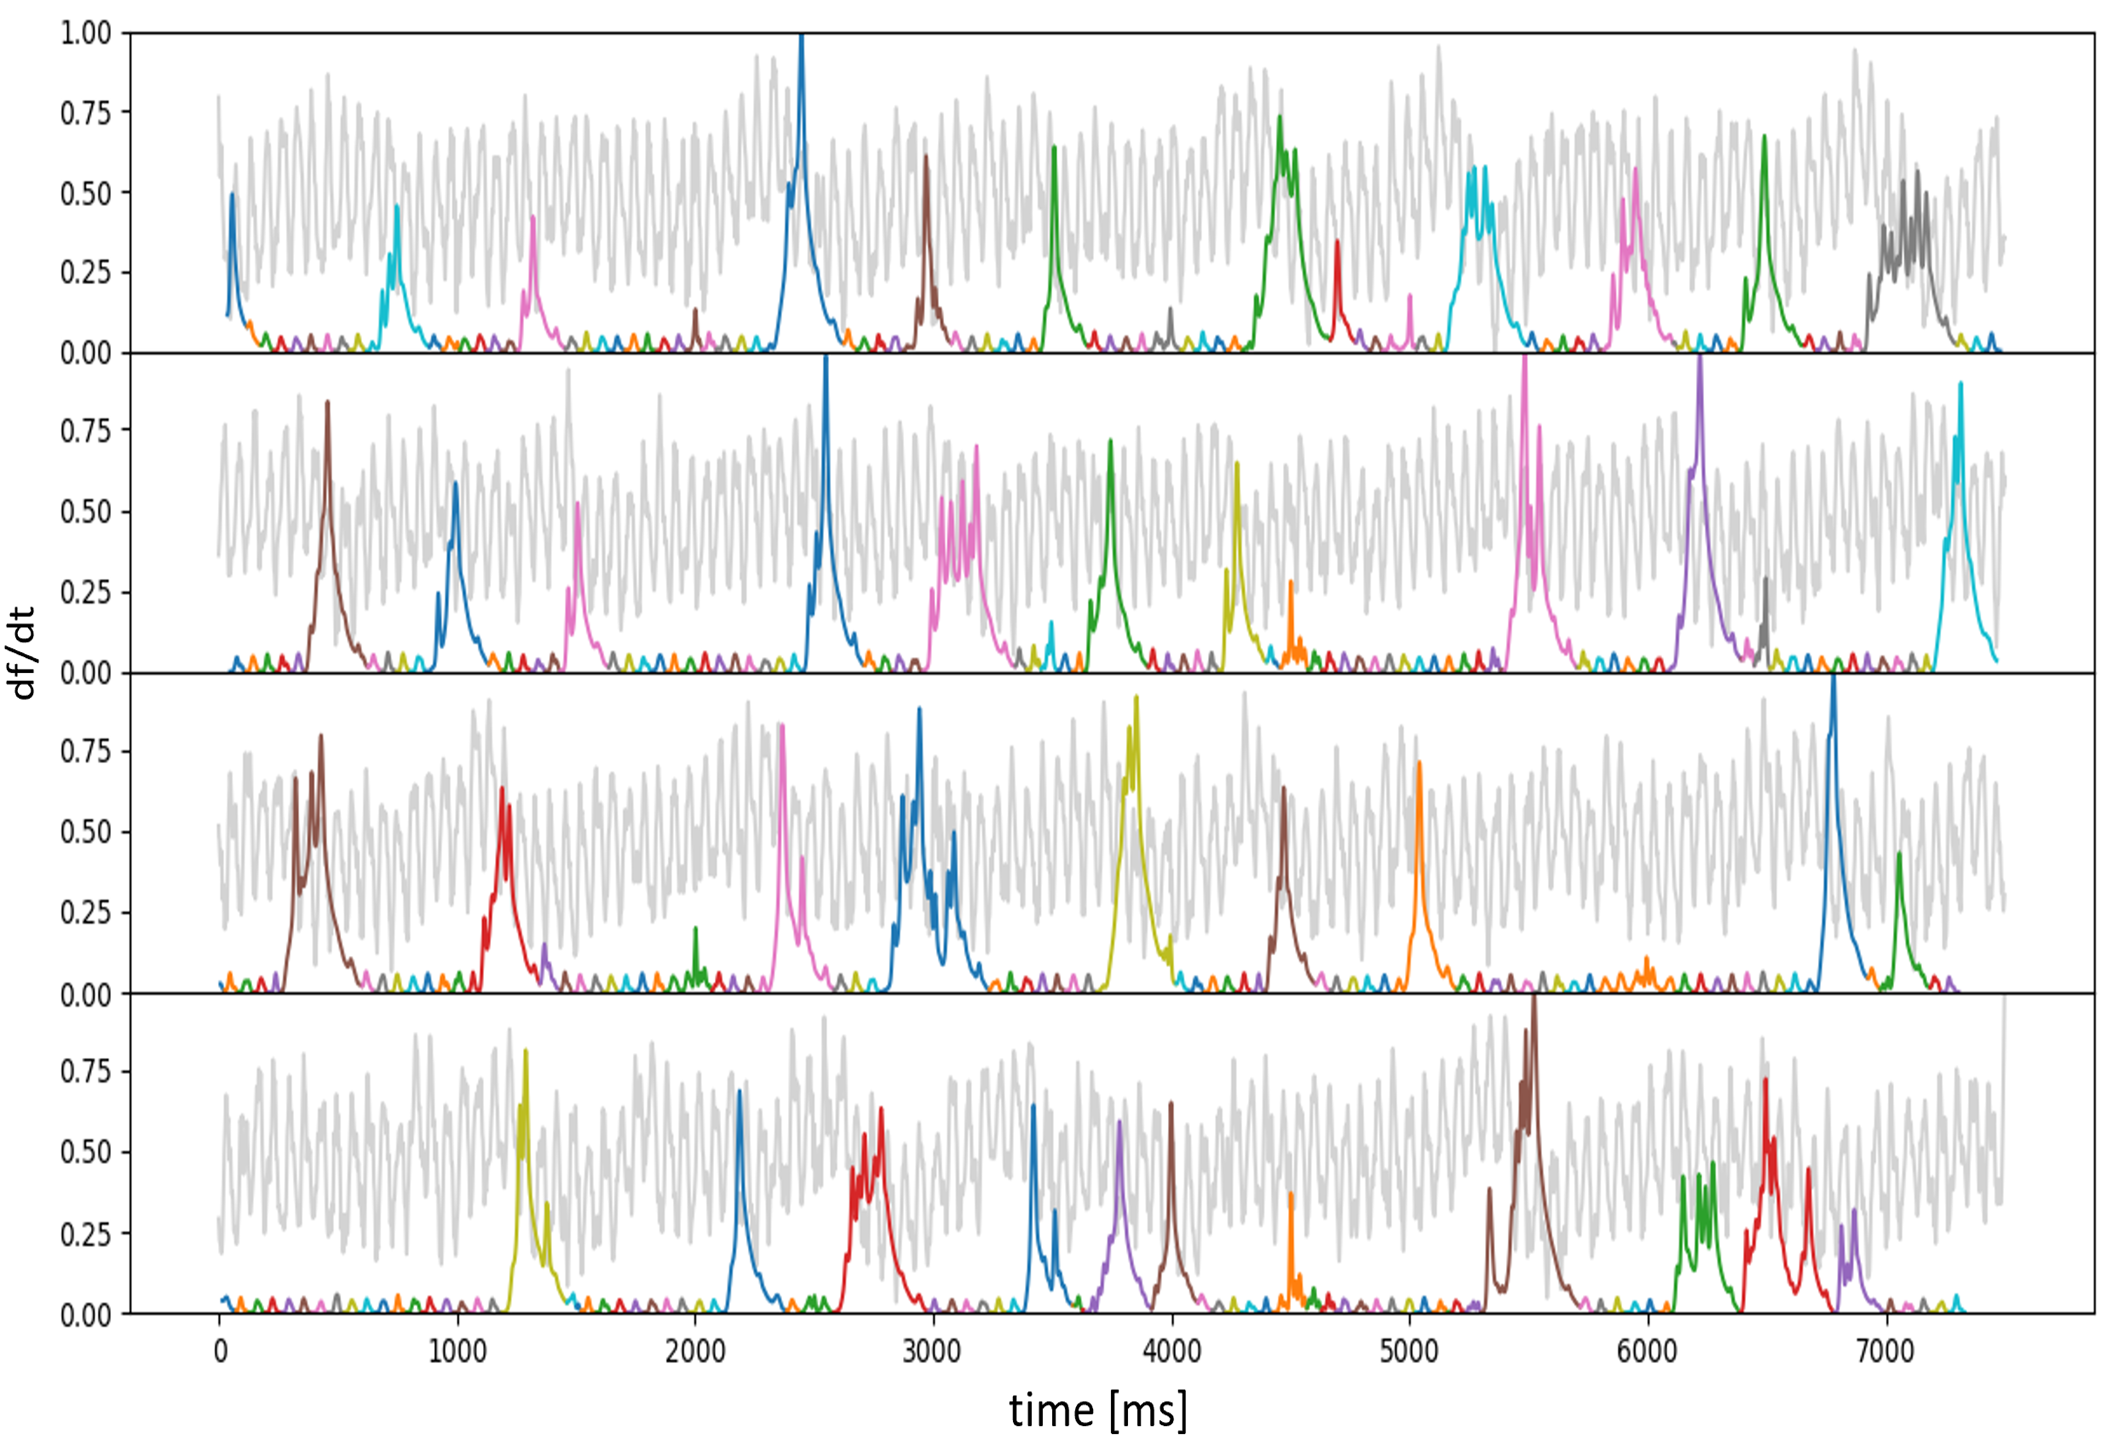
\includegraphics[width=\textwidth,height=\textheight,keepaspectratio]{Figures/slow_wave_segmentation}
\decoRule
\caption[Detected slow waves for a sample recording]{Detected slow waves for a sample recording at 1.8\% isoflurane.}
\label{fig:slow_wave_segmentation}
\end{figure}

\begin{figure}[!htb]
\centering
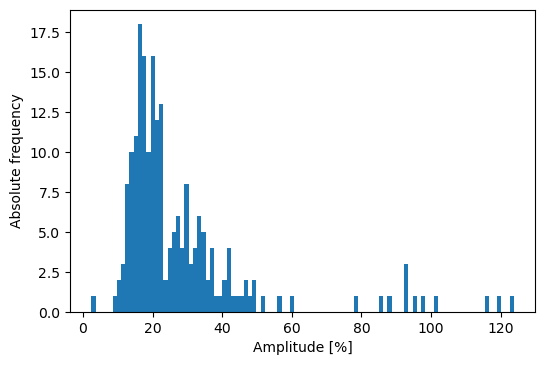
\includegraphics[width=\textwidth,height=\textheight,keepaspectratio]{Figures/selected_waves_distribution_of_peak_amplitude}
\decoRule
\caption[Distribution of the peak amplitude of detected waves]{Distribution of the peak amplitude of detected waves.}
\label{fig:selected_waves_distribution_of_peak_amplitude}
\end{figure}

\begin{figure}[!htb]
\centering
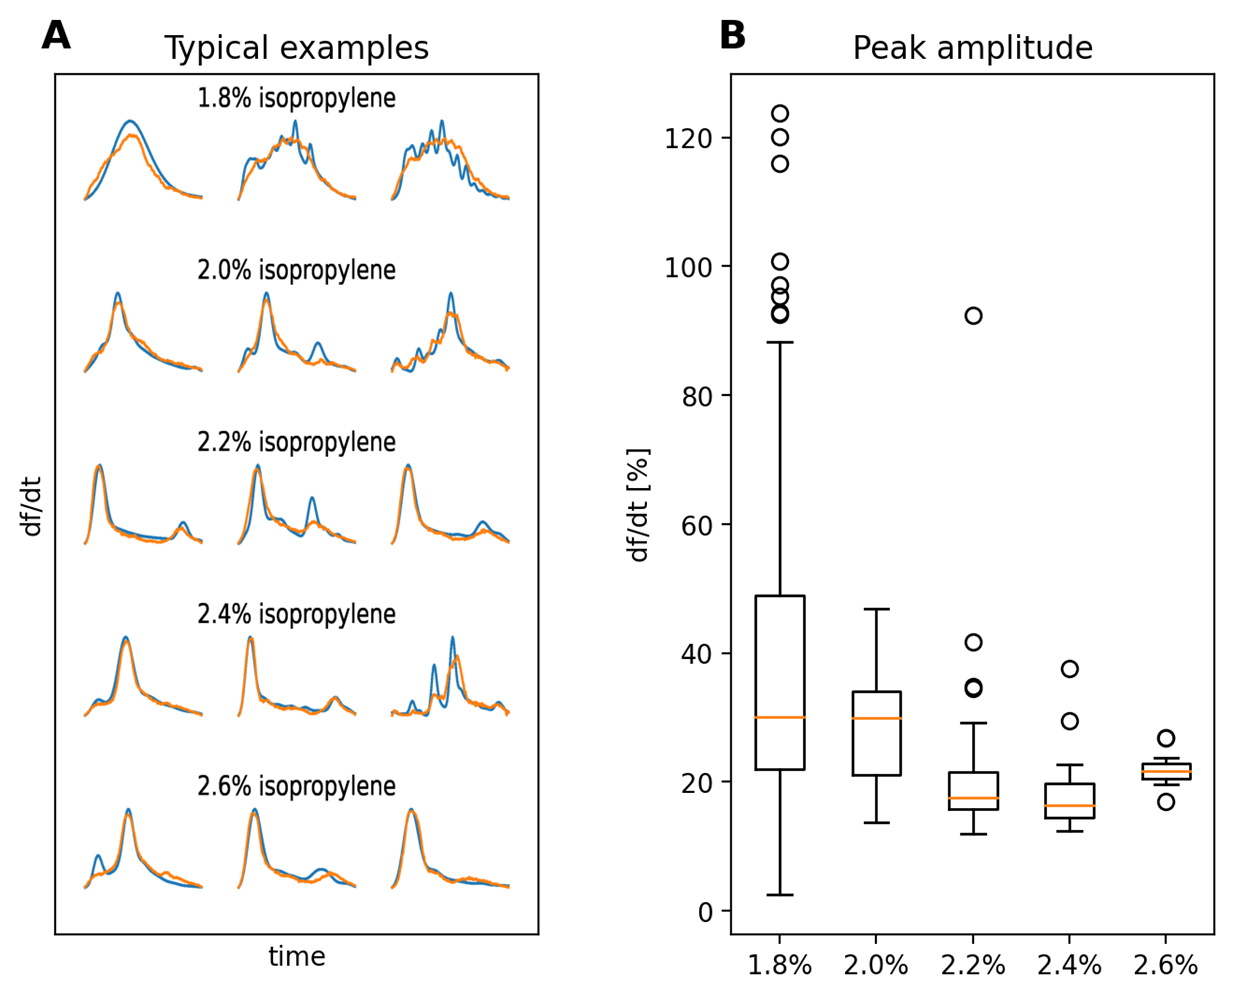
\includegraphics[width=\textwidth,height=\textheight,keepaspectratio]{Figures/typical_examples_and_peak_amplitudes}
\decoRule
\caption[Typical examples and peak amplitudes]{Typical examples and peak amplitudes.}
\label{fig:typical_examples_and_peak_amplitudes}
\end{figure}

\begin{figure}[!htb]
\centering
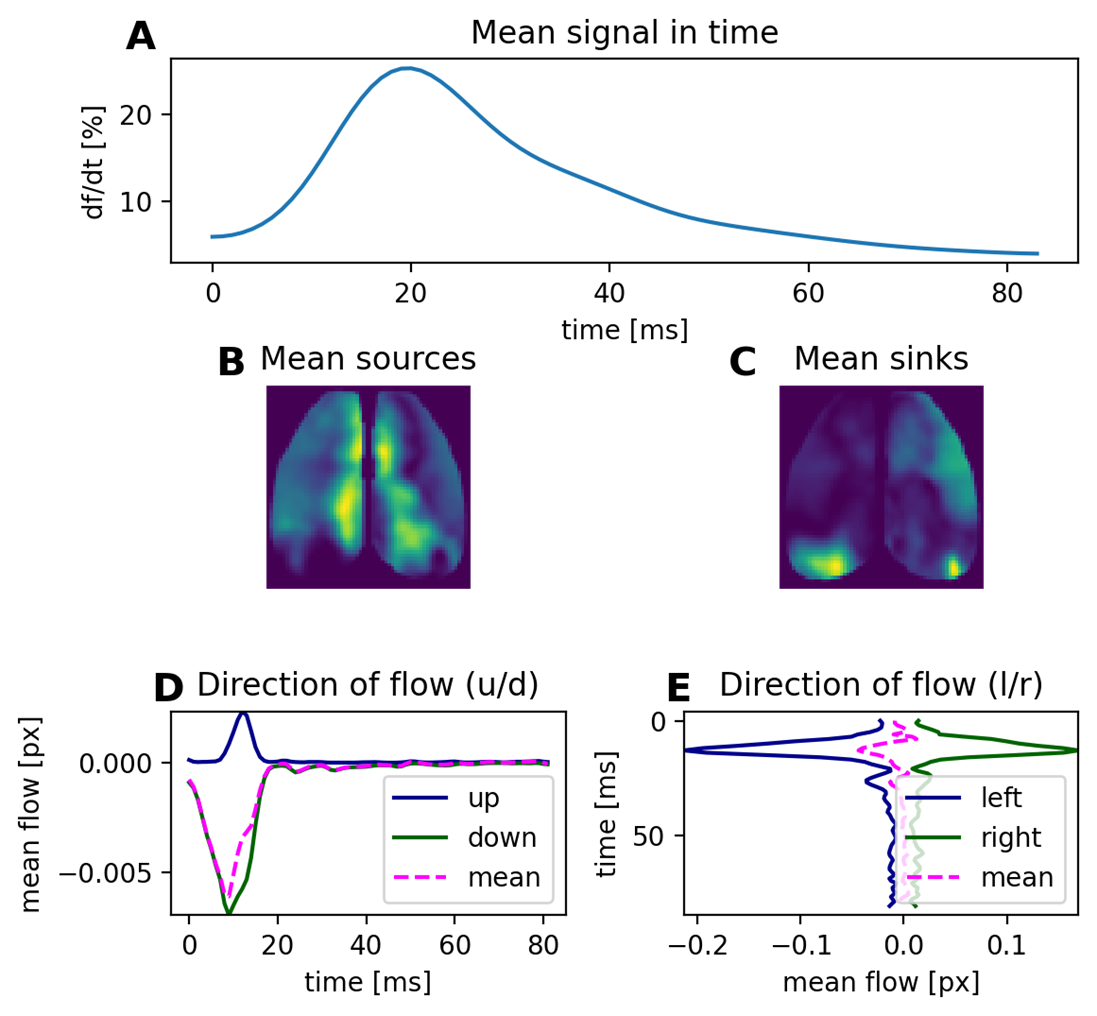
\includegraphics[width=\textwidth,height=\textheight,keepaspectratio]{Figures/percentage_change_direction_of_flow_and_sources_sinks}
\decoRule
\caption[Percentage change, direction of flow and the distibibution of sources and sinks for a typical example]{Percentage change, direction of flow and the distibibution of sources and sinks for a typical example with one peak.}
\label{fig:percentage_change_direction_of_flow_and_sources_sinks}
\end{figure}


\begin{figure}[!htb]
\centering
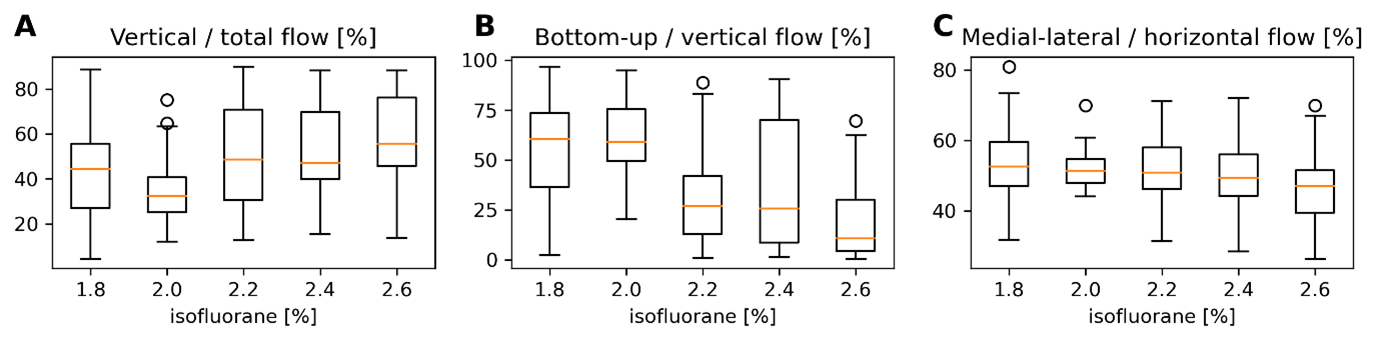
\includegraphics[width=\textwidth,height=\textheight,keepaspectratio]{Figures/direction_per_isoflourane}
\decoRule
\caption[Direction of flow for different levels of isoflurane]{The direction of flow for different levels of isoflurane.}
\label{fig:direction_per_isoflourane}
\end{figure}

\begin{figure}[!htb]
\centering
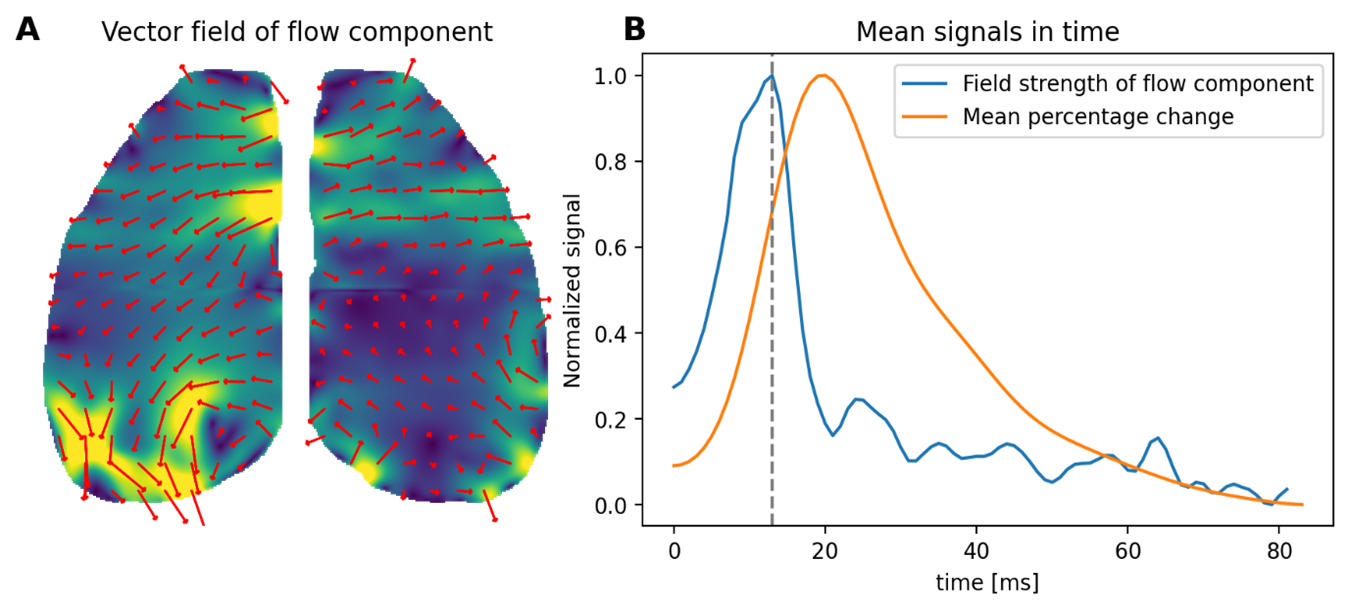
\includegraphics[width=\textwidth,height=\textheight,keepaspectratio]{Figures/vector_field_flow_component}
\decoRule
\caption[A sample vector field and field strength of flow in time.]{A sample vector field and field strength of flow in time.}
\label{fig:vector_field_flow_component}
\end{figure}

\begin{figure}[!htb]
\centering
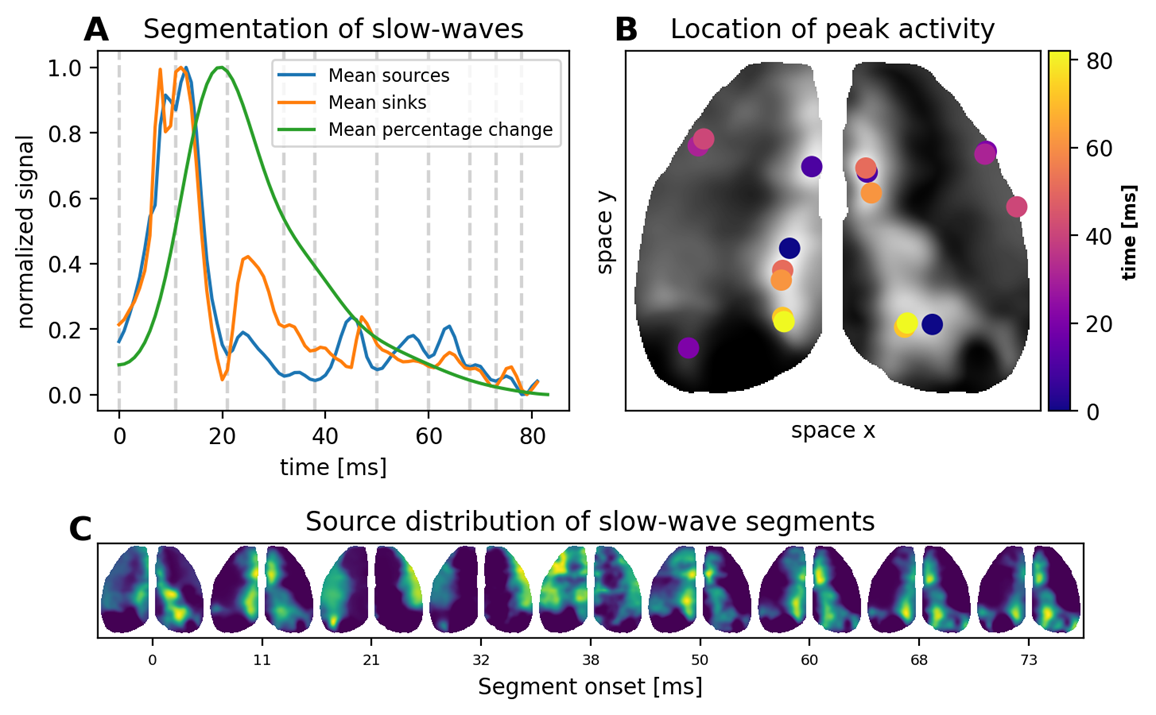
\includegraphics[width=\textwidth,height=\textheight,keepaspectratio]{Figures/slow_wave_subsegements}
\decoRule
\caption[Slow wave subsegments]{Slow wave subsegments}
\label{fig:slow_wave_subsegements}
\end{figure}

\begin{figure}[!htb]
\centering
\includegraphics[width=\textwidth,height=\textheight,keepaspectratio]{Figures/sources_are_not_mean_signal}
\decoRule
\caption[Sources are not the mean signal]{Sources are not the mean signal}
\label{fig:sources_are_not_mean_signal}
\end{figure}


\section{Main Section 1}

Lorem ipsum dolor sit amet, consectetur adipiscing elit. Aliquam ultricies lacinia euismod. Nam tempus risus in dolor rhoncus in interdum enim tincidunt. Donec vel nunc neque. In condimentum ullamcorper quam non consequat. Fusce sagittis tempor feugiat. Fusce magna erat, molestie eu convallis ut, tempus sed arcu. Quisque molestie, ante a tincidunt ullamcorper, sapien enim dignissim lacus, in semper nibh erat lobortis purus. Integer dapibus ligula ac risus convallis pellentesque.

%-----------------------------------
%	SUBSECTION 1
%-----------------------------------
\subsection{Reconstruction manifolds and latent space distributions}

\begin{figure}[!htb]
\centering
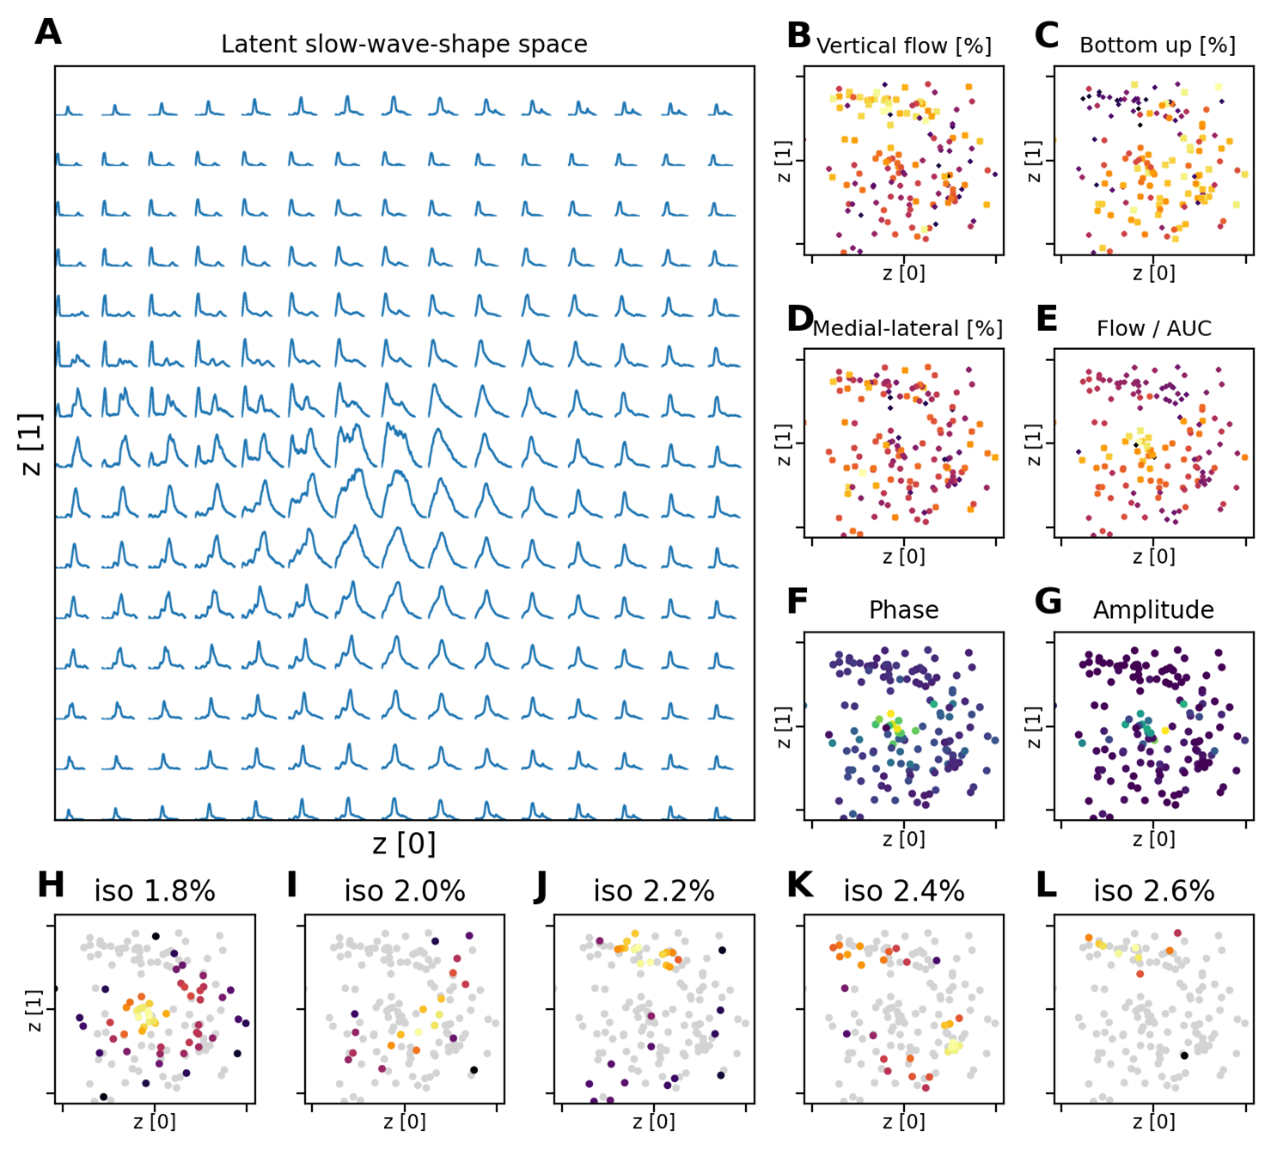
\includegraphics[width=\textwidth,height=\textheight,keepaspectratio]{Figures/slow_wave_shape_space}
\decoRule
\caption[Latent slow wave shape space]{Latent slow wave shape space}
\label{fig:slow_wave_shape_space}
\end{figure}


\begin{figure}[!htb]
\centering
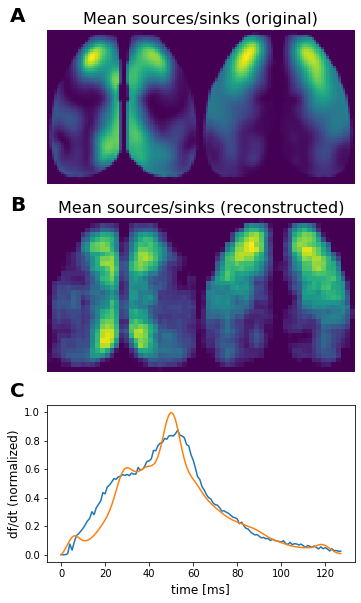
\includegraphics[width=\textwidth,height=\textheight,keepaspectratio]{Figures/reconstructions_example_mixed_input}
\decoRule
\caption[Examples for reconstructions of the mixed input model]{Examples for reconstructions of the mixed input model}
\label{fig:reconstructions_example_mixed_input}
\end{figure}

\begin{figure}[!htb]
\centering
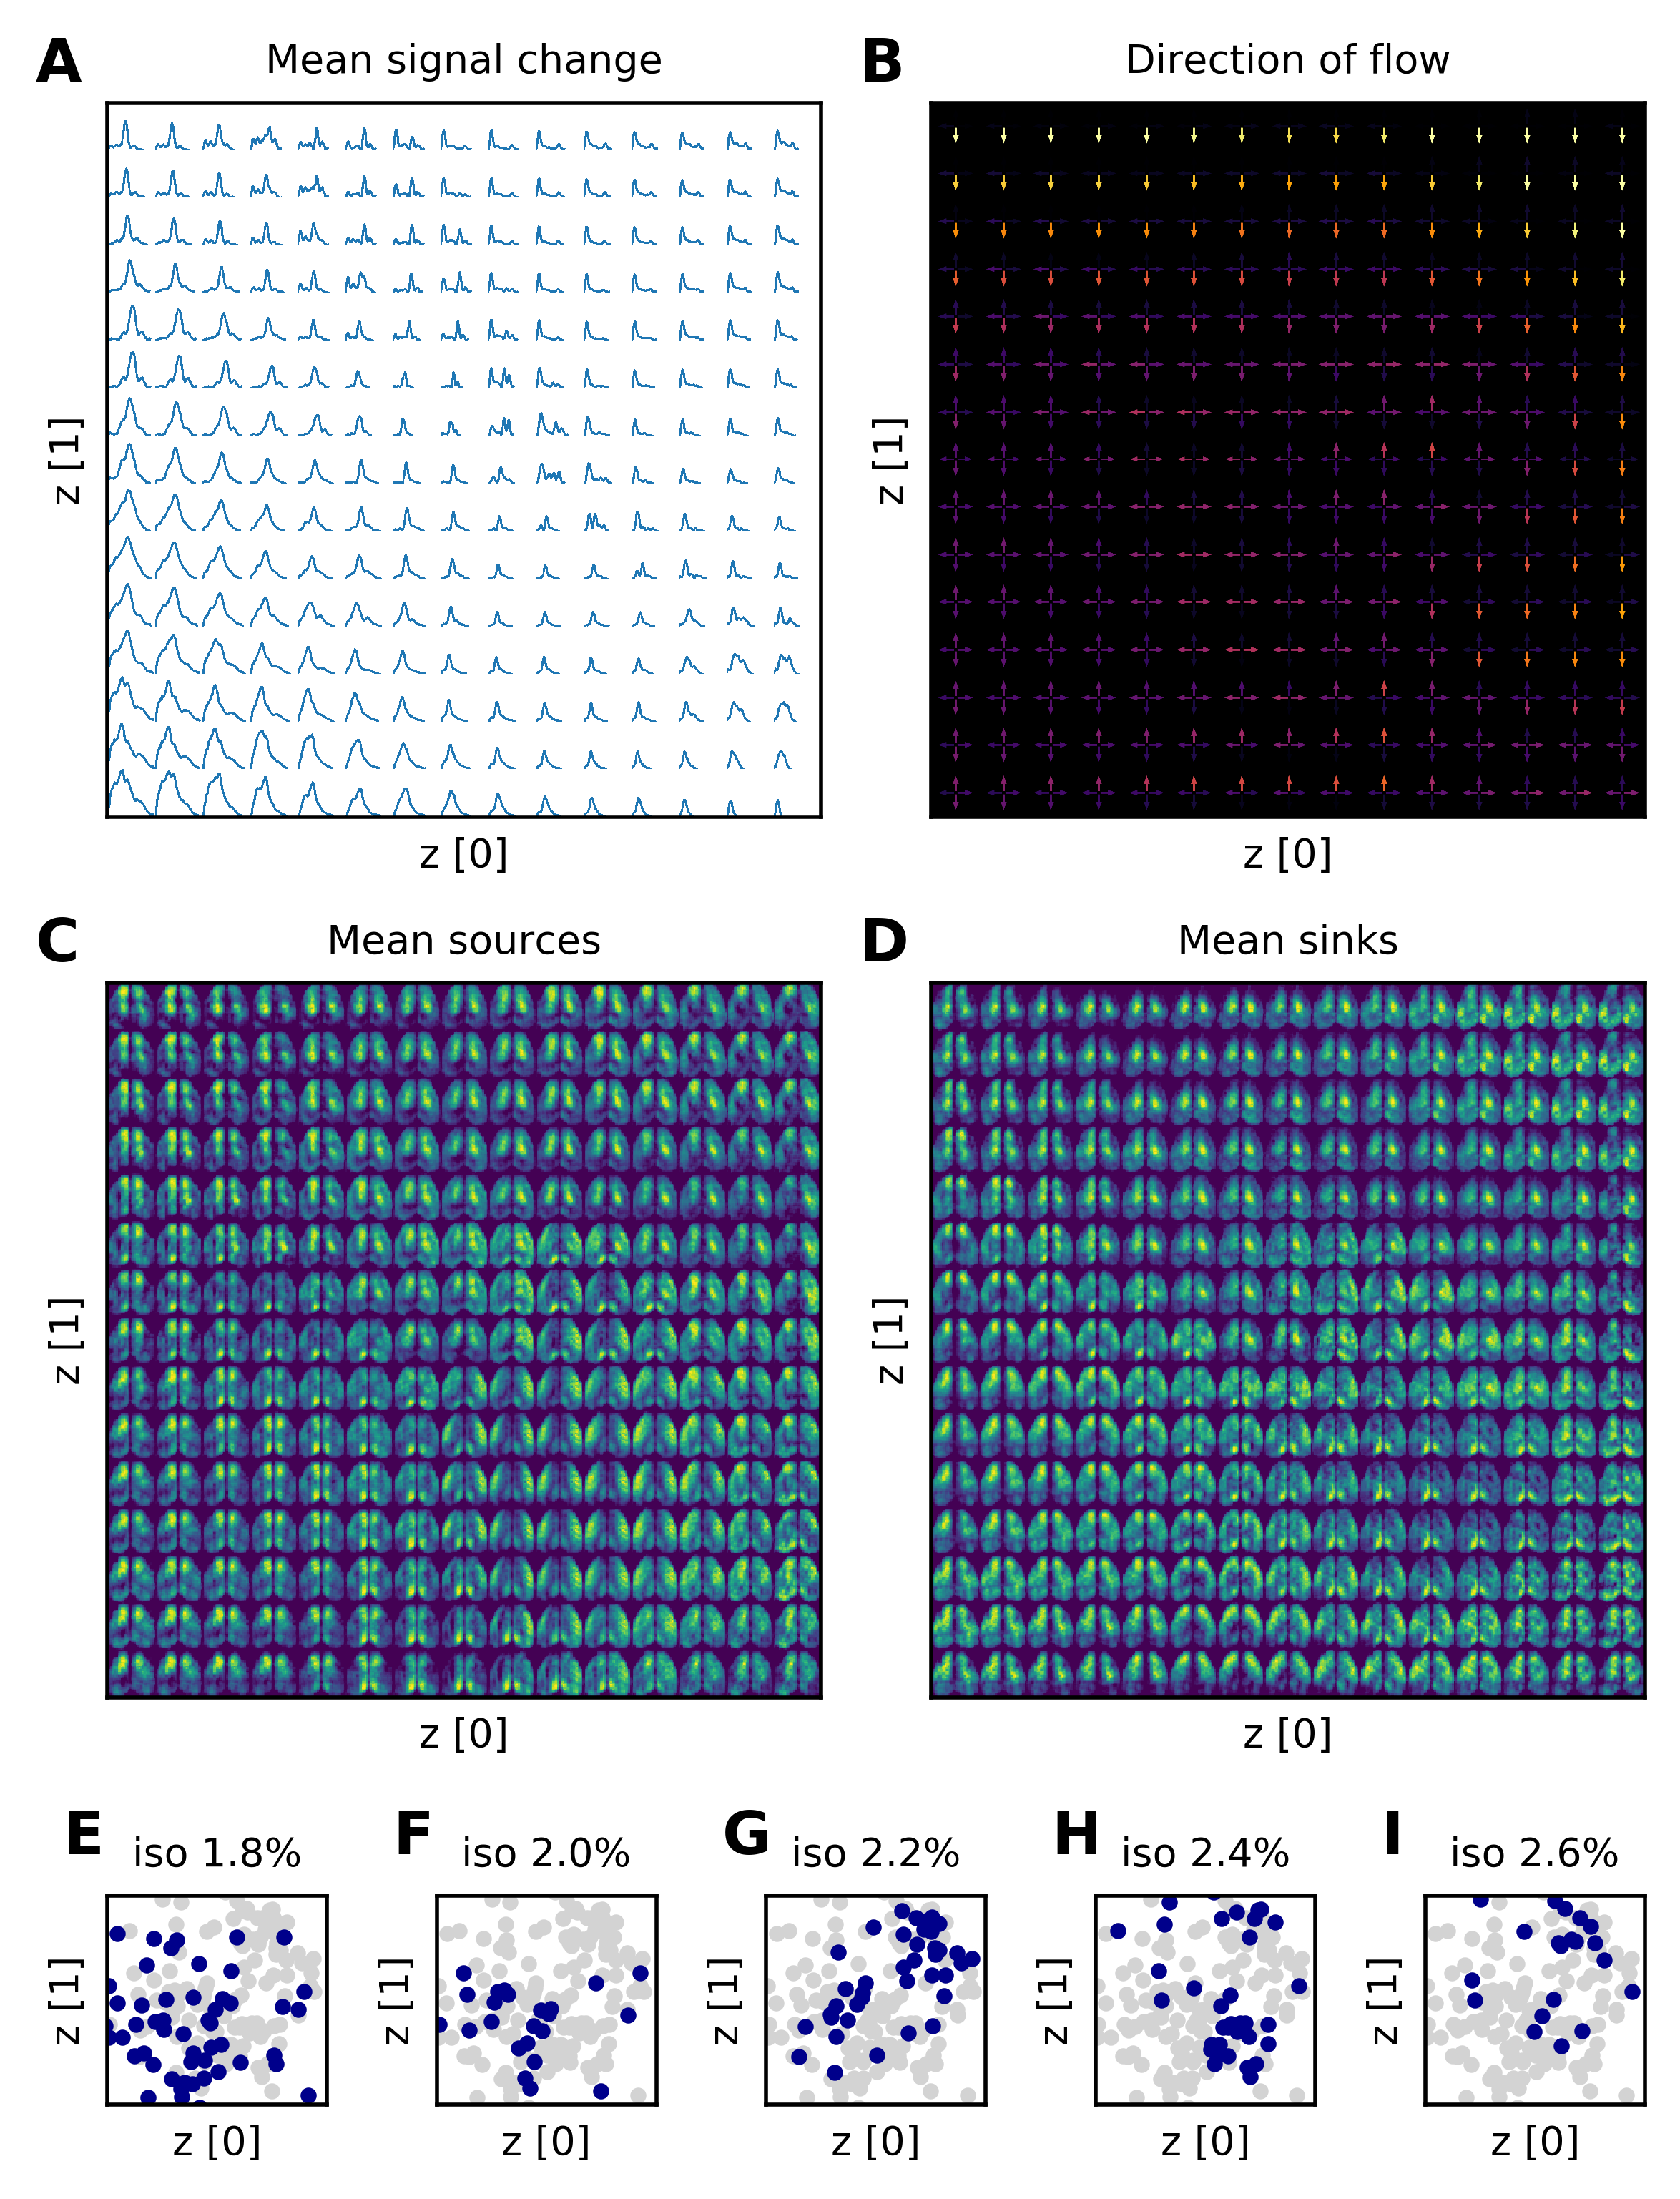
\includegraphics[width=\textwidth,height=\textheight,keepaspectratio]{Figures/latent_slow_wave_space}
\decoRule
\caption[Latent slow wave space]{Latent slow wave space}
\label{fig:latent_slow_wave_space}
\end{figure}

\begin{figure}[!htb]
\centering
\includegraphics[width=\textwidth,height=\textheight,keepaspectratio]{Figures/latent_flow_space}
\decoRule
\caption[Latent flow space]{Latent flow space}
\label{fig:latent_flow_space}
\end{figure}

Nunc posuere quam at lectus tristique eu ultrices augue venenatis. Vestibulum ante ipsum primis in faucibus orci luctus et ultrices posuere cubilia Curae; Aliquam erat volutpat. Vivamus sodales tortor eget quam adipiscing in vulputate ante ullamcorper. Sed eros ante, lacinia et sollicitudin et, aliquam sit amet augue. In hac habitasse platea dictumst.

%-----------------------------------
%	SUBSECTION 2
%-----------------------------------

\subsection{Subsection 2}
Morbi rutrum odio eget arcu adipiscing sodales. Aenean et purus a est pulvinar pellentesque. Cras in elit neque, quis varius elit. Phasellus fringilla, nibh eu tempus venenatis, dolor elit posuere quam, quis adipiscing urna leo nec orci. Sed nec nulla auctor odio aliquet consequat. Ut nec nulla in ante ullamcorper aliquam at sed dolor. Phasellus fermentum magna in augue gravida cursus. Cras sed pretium lorem. Pellentesque eget ornare odio. Proin accumsan, massa viverra cursus pharetra, ipsum nisi lobortis velit, a malesuada dolor lorem eu neque.

%----------------------------------------------------------------------------------------
%	SECTION 2
%----------------------------------------------------------------------------------------

\section{Main Section 2}

Sed ullamcorper quam eu nisl interdum at interdum enim egestas. Aliquam placerat justo sed lectus lobortis ut porta nisl porttitor. Vestibulum mi dolor, lacinia molestie gravida at, tempus vitae ligula. Donec eget quam sapien, in viverra eros. Donec pellentesque justo a massa fringilla non vestibulum metus vestibulum. Vestibulum in orci quis felis tempor lacinia. Vivamus ornare ultrices facilisis. Ut hendrerit volutpat vulputate. Morbi condimentum venenatis augue, id porta ipsum vulputate in. Curabitur luctus tempus justo. Vestibulum risus lectus, adipiscing nec condimentum quis, condimentum nec nisl. Aliquam dictum sagittis velit sed iaculis. Morbi tristique augue sit amet nulla pulvinar id facilisis ligula mollis. Nam elit libero, tincidunt ut aliquam at, molestie in quam. Aenean rhoncus vehicula hendrerit.
